% small.tex
\documentclass[12pt]{beamer}
\usetheme{amcg}
\beamertemplatenavigationsymbolsempty
\renewcommand{\thefootnote}{}
\providecommand{\e}[1]{\ensuremath{\times 10^{#1}}}
\usepackage{mathptmx}
\usepackage{helvet}
\newcommand\TILDE{\char`\~}
\usepackage{listings}
\lstset{
        basicstyle              = \scriptsize\ttfamily,
        breaklines              = true,
        breakindent             = 10pt,
        breakatwhitespace       = true,
        breakautoindent         = true,
        keywordstyle            = \color[RGB]{0,0,255},
        commentstyle            = \itshape\color[RGB]{120,120,120},
        stringstyle             = \color[rgb]{0.627,0.126,0.941},
        emphstyle               = {[0]\color[RGB]{236,0,168}},
        emphstyle               = {[1]\color[RGB]{34,139,34}\underbar},
        emphstyle               = {[2]\textbf}
}
% items enclosed in square brackets are optional; explanation below
\title[Running]{Running Fluidity and Visualising the Results}
\subtitle[]{}
\institute{1 - Dept of Earth Science and Engineering, Imperial College London}
\author[Jon Hill]{\large{Jon Hill}\inst{1}}
\date{}
\AtBeginSection[]
{
   \begin{frame}
       \frametitle{Outline}
       \tableofcontents[currentsection]
   \end{frame}
}


\begin{document}


%--- the titlepage frame -------------------------%
\begin{frame}
  \titlepage
\end{frame}

%-- Overview slide --- %
\section*{Outline}
\begin{frame}
  \frametitle{Outline}
  \tableofcontents
\end{frame}

\section{Running}
\begin{frame}
    \frametitle{Running Fluidity}

    \texttt{./fluidity}

\end{frame}
\begin{frame}[fragile]
    \frametitle{Running Fluidity}
\lstset{language=bash,basicstyle=\tiny}
\begin{lstlisting}[language=bash]

Revision: fluidity/4.1
Compile date: Nov 20 2012 10:16:12
OpenMP Support			no
Adaptivity support		yes
...
FEMDEM support			no
Hyperlight support		no


Usage: fluidity [options ...] [simulation-file]

Options:
 -h, --help
	Help! Prints this message.
 -l, --log
	Create log file for each process (useful for non-interactive testing).
 -v <level>, --verbose
	Verbose output to stdout, default level 0
 -p, --profile
	Print profiling data at end of run
	This provides aggregated elapsed time for coarse-level computation
	(Turned on automatically if verbosity is at level 2 or above)
 -V, --version
	Version
\end{lstlisting}
\end{frame}

\begin{frame}
    \frametitle{Running Fluidity}

\texttt{./fluidity my.flml}

\texttt{./fluidity -l my.flml}

\texttt{./fluidity -l -v3 my.flml}
\end{frame}


\section{Output}

\subsection{Filetypes and tools}
\begin{frame}
    \frametitle{Filetypes}
There are \textbf{two} main filetypes:
\begin{itemize}
    \item .stat file
    \item Unstructured VTK file (.vtu or .pvtu)
\end{itemize}
\vspace{5mm}
You may also have log files:
\begin{itemize}
    \item fluidity.log.*
    \item fluidity.err.*
\end{itemize}

\end{frame}

\begin{frame}
    \frametitle{Tools}
\begin{itemize}
\item Statplot
\item Paraview
\item Python
    \begin{itemize}
    \item vtktools
    \item fluidity.statparser
    \end{itemize}
\end{itemize}
\end{frame}

\subsection{The stat file}

\begin{frame}
    \frametitle{The stat file}
\begin{columns}
\begin{column}{0.6\textwidth}
\begin{itemize}
\item Bespoke data file type
\item Various tools to read and process these data
\item Either ASCII or binary
\end{itemize}
\end{column}
\begin{column}{0.4\textwidth}
\begin{center}
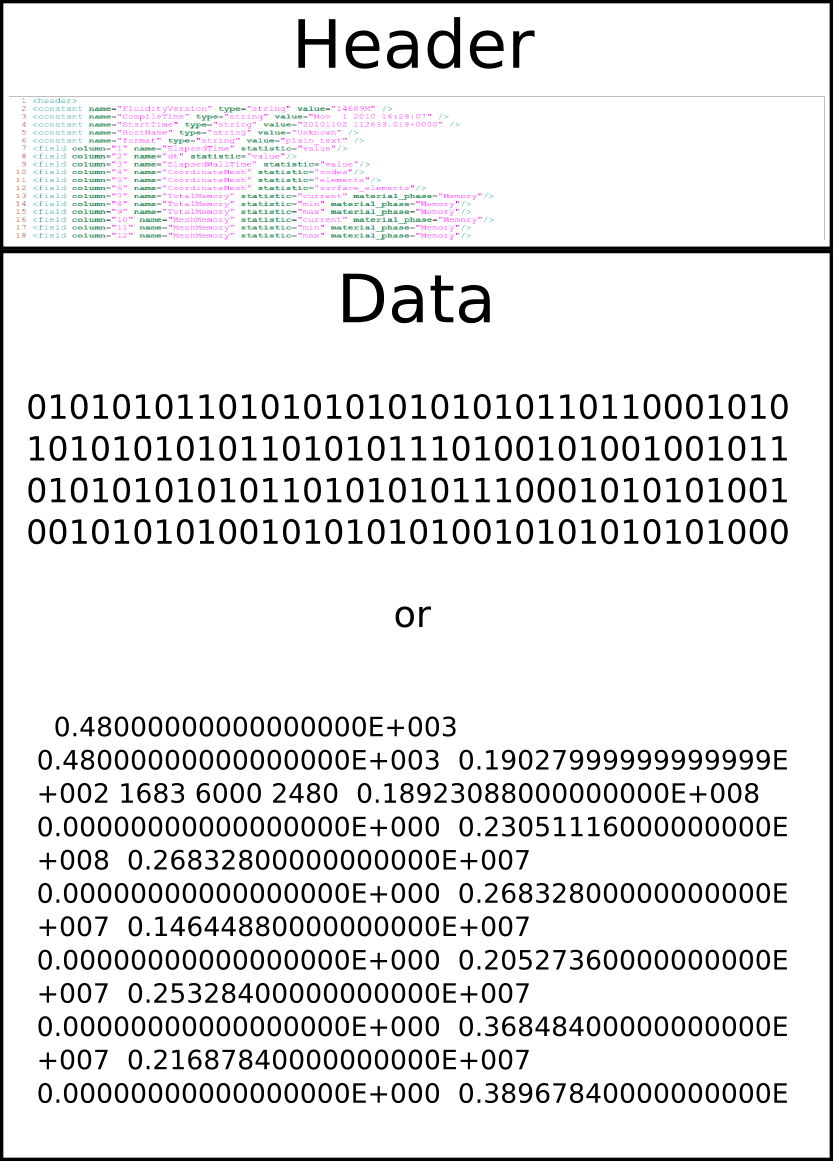
\includegraphics[width=0.7\textwidth]{images/stat_file.png}
\end{center}
\end{column}
\end{columns}
\end{frame}

\begin{frame}
    \frametitle{Statplot}
\begin{center}
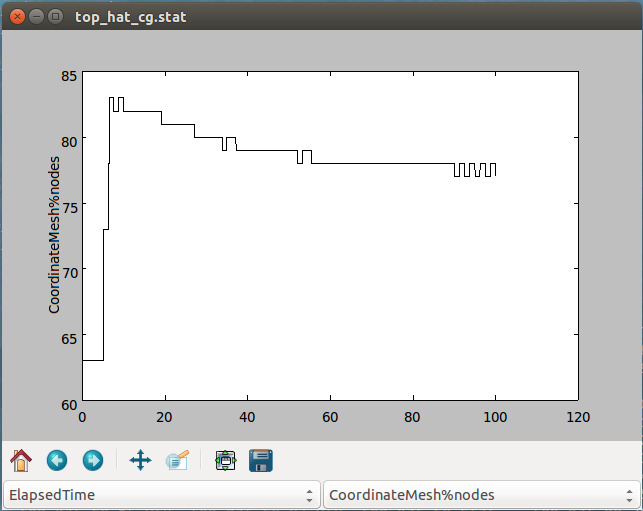
\includegraphics[width=0.8\textwidth]{images/statplot.png}
\end{center}
Usage: \texttt{\TILDE/fluidity/bin/statplot my\_statfile.stat}
\end{frame}

\begin{frame}
    \frametitle{Statplot}
\begin{center}
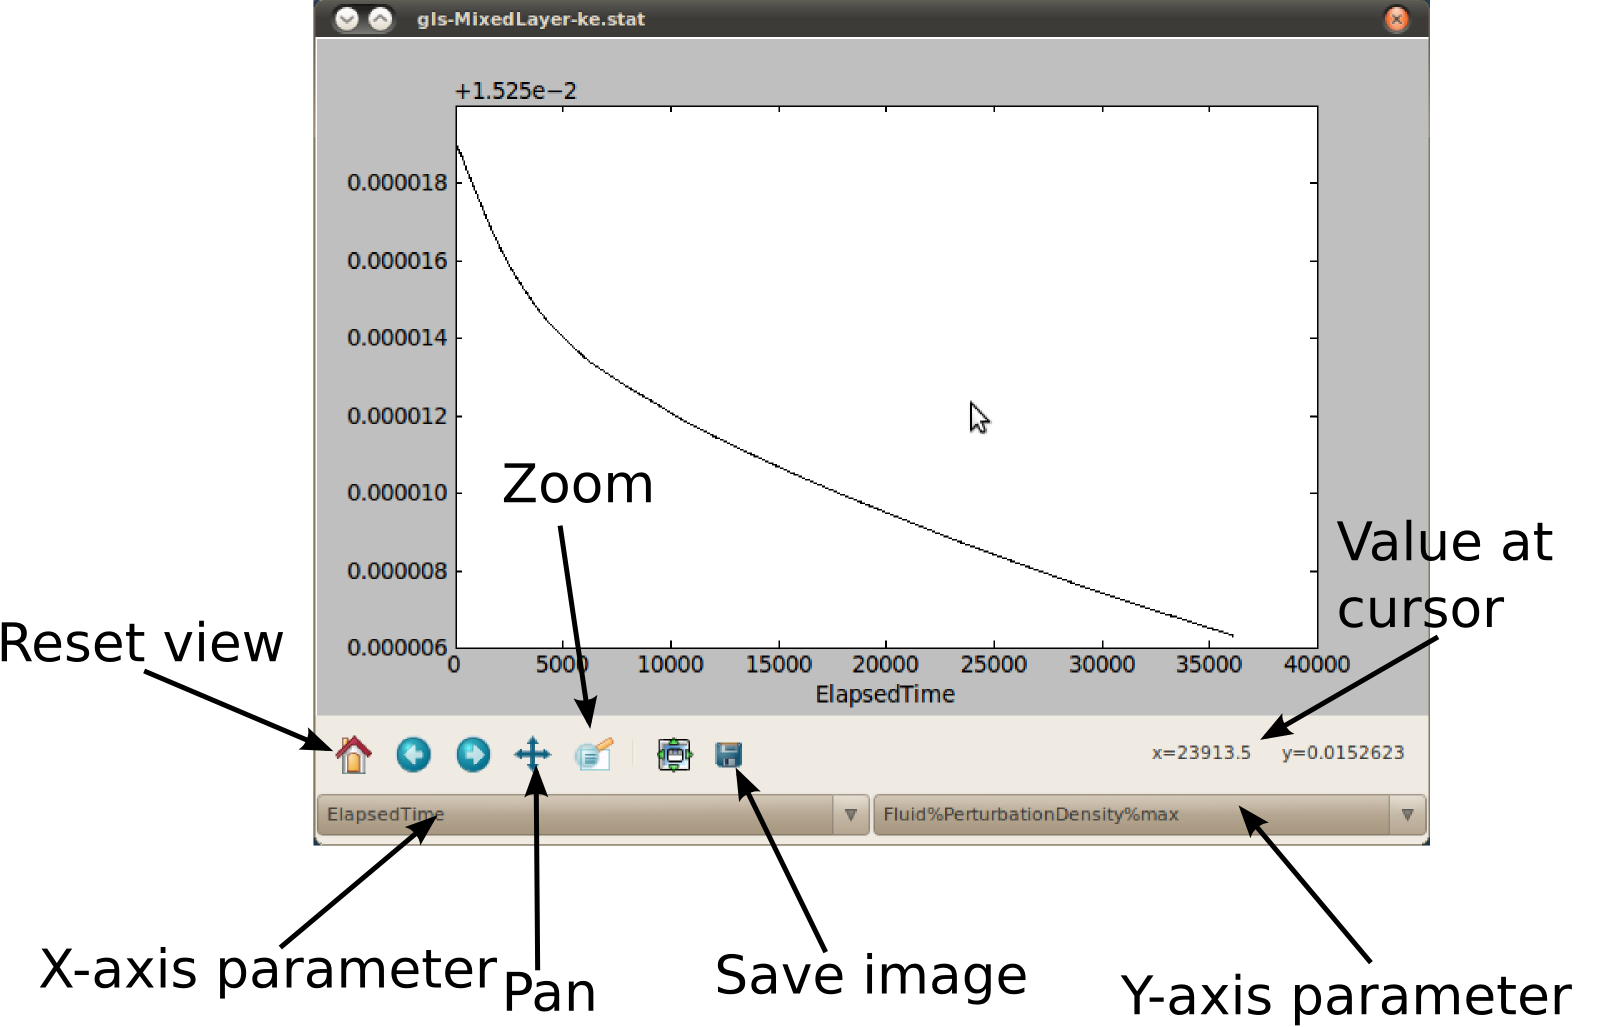
\includegraphics[width=0.8\textwidth]{images/statplot_labelled.png}
\end{center}
\end{frame}

\begin{frame}
    \frametitle{Statplot keys}
\begin{itemize}
\item s - scatter plot
\item l - line plot
\item r - refresh data
\item R - refersh data, but keep current bounds
\item x - switch x-axis from linear to log or vice versa
\item y - switch y-axis from linear to log or vice versa
\item q - quit (note: \textbf{no warnings!})
\end{itemize}
\end{frame}

\begin{frame}
    \frametitle{Statplot example}
Open the stat file at from your advection problem

Things to try:
\begin{itemize}
\item Switch between scatter plot and line plot views
\item Change the graph to show the number of elements through the run
\item Plot velocity magnitude minimum against velocity magnitude maximum
\item Zoom in and save a small part of the plot to file
\end{itemize}
\end{frame}


\subsection{Paraview}
\begin{frame}
    \frametitle{Paraview}
Open-source scientific visualisation software from KitView
\begin{center}
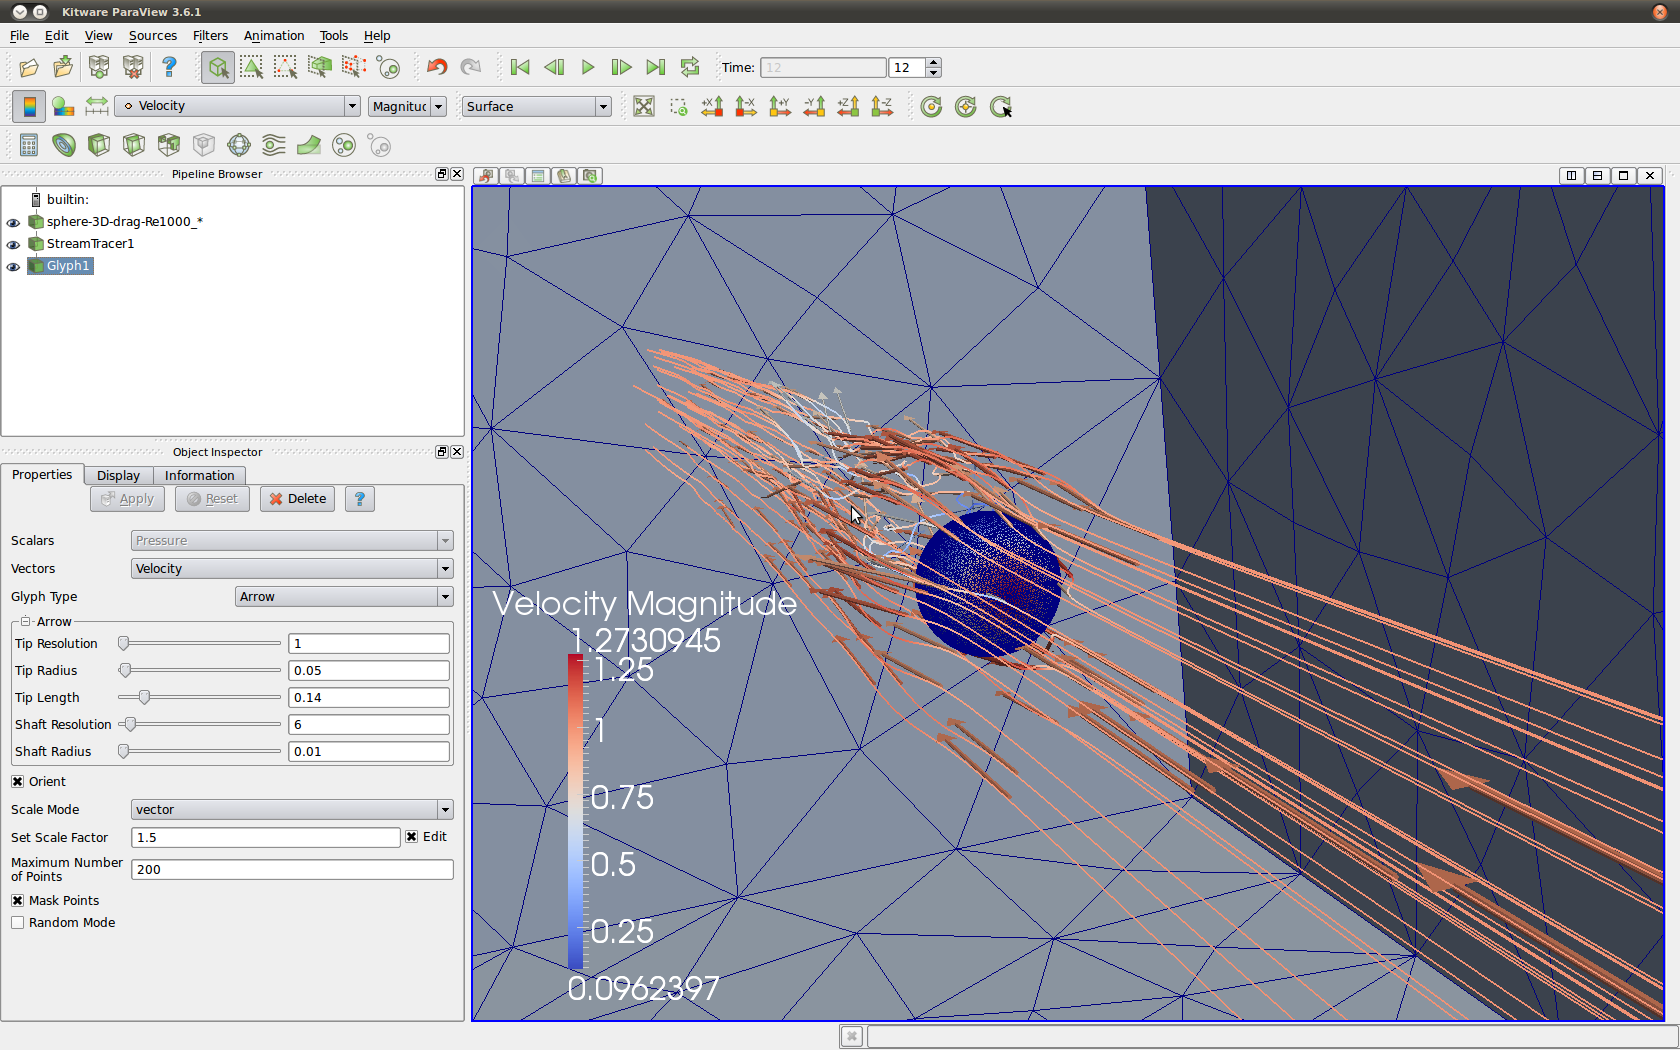
\includegraphics[width=0.7\textwidth]{images/paraview_example.png}
\end{center}
\end{frame}

\begin{frame}
    \frametitle{Paraview: main window}
\begin{center}
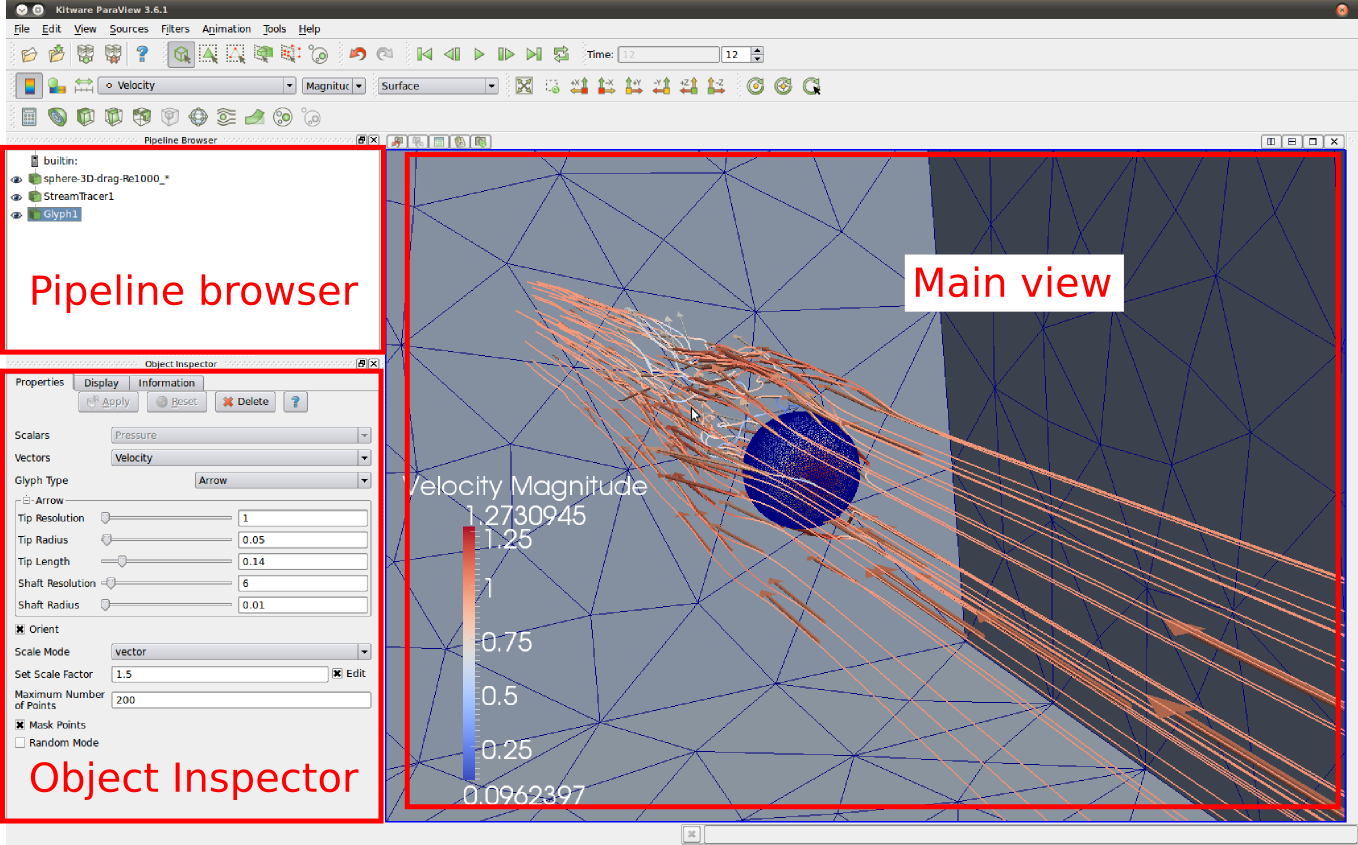
\includegraphics[width=0.8\textwidth]{images/paraview_window.png}
\end{center}
\end{frame}
\begin{frame}
    \frametitle{Paraview: main window}
\begin{center}
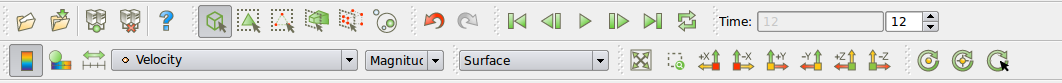
\includegraphics[width=\textwidth]{images/paraview_toolbar.png}
\end{center}
\end{frame}
\begin{frame}
    \frametitle{Paraview: main window}
\begin{center}
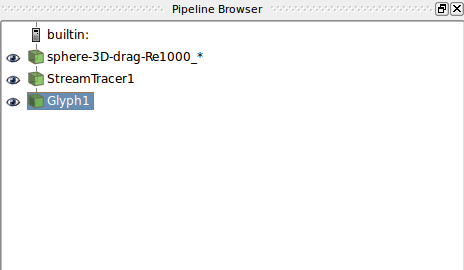
\includegraphics[width=0.7\textwidth]{images/paraview_pipeline.png}
\end{center}
\end{frame}
\begin{frame}
    \frametitle{Paraview: main window}
\begin{center}
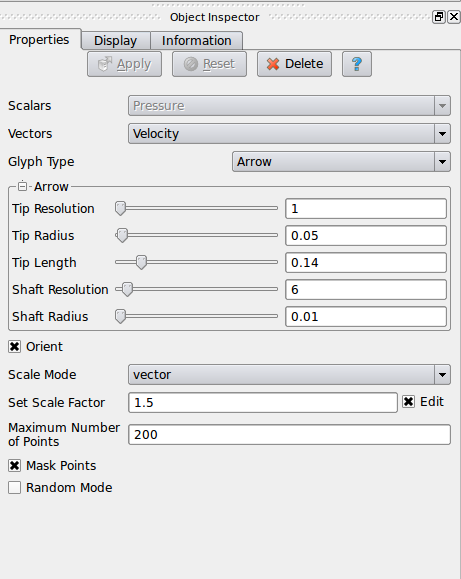
\includegraphics[width=0.5\textwidth]{images/paraview_object.png}
\end{center}
\end{frame}

\begin{frame}
    \frametitle{Paraview}
\begin{center}
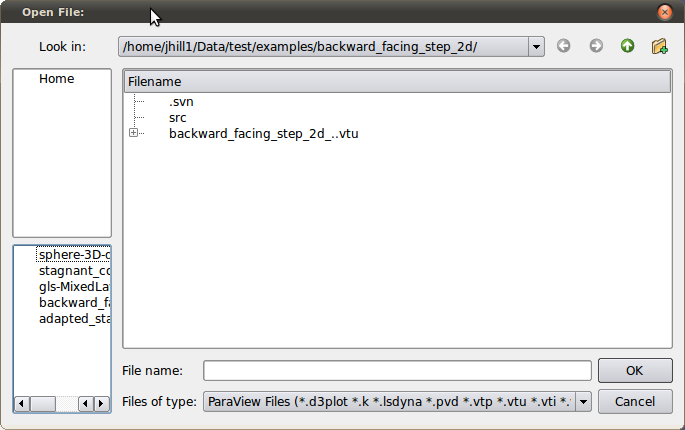
\includegraphics[width=0.8\textwidth]{images/paraview_open.png}
\end{center}
\end{frame}
\begin{frame}
    \frametitle{Paraview}
\begin{center}
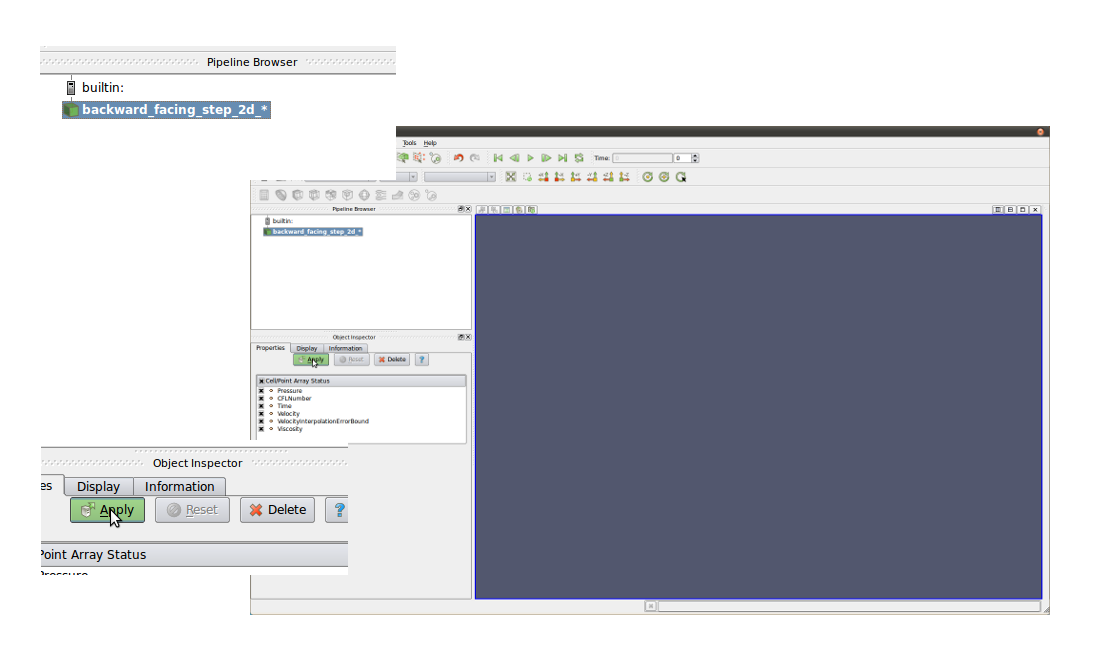
\includegraphics[width=\textwidth]{images/paraview_after_open.png}
\end{center}
\end{frame}
\begin{frame}
    \frametitle{Paraview}
\begin{center}
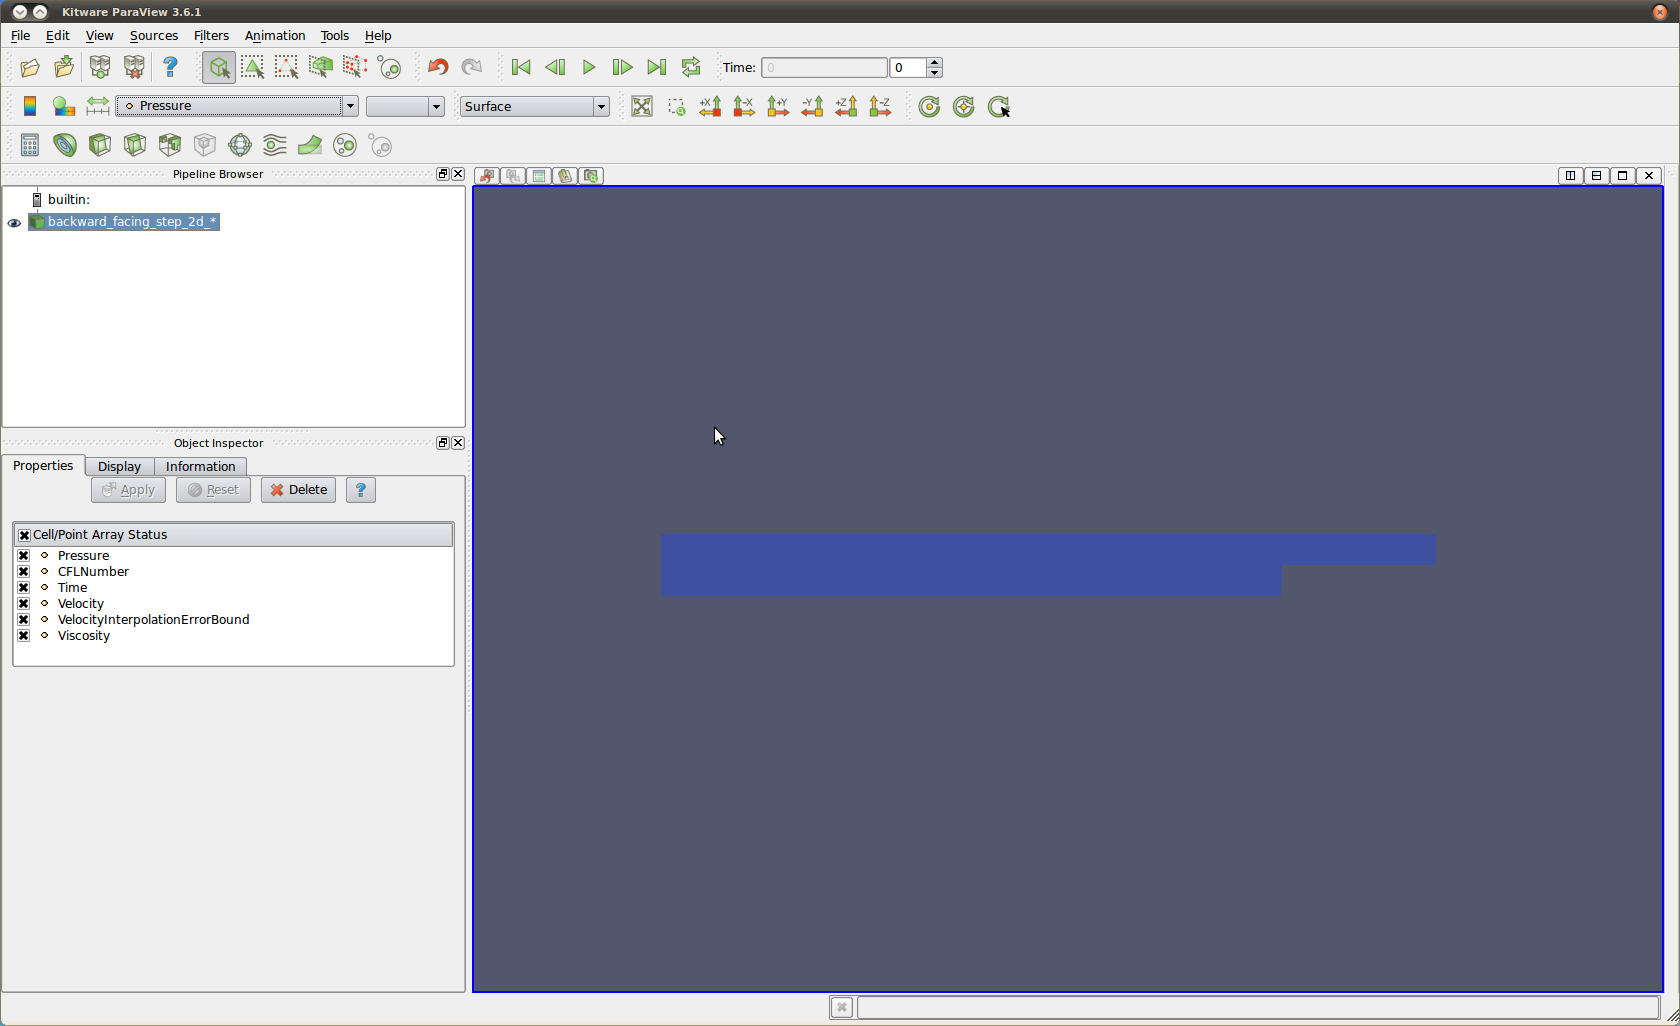
\includegraphics[width=0.75\textwidth]{images/paraview_after_loading.png}
\end{center}
\end{frame}
\begin{frame}
    \frametitle{Paraview}
\begin{itemize}
\item Right click: Zoom-in and out
\item Left-click: rotate
\item Middle-button: move
\item Zoom in and save a small part of the plot to file
\end{itemize}
\end{frame}

\begin{frame}
	\frametitle{Animations}
\begin{enumerate}
\item File $\rightarrow$ Save Animation
\item Set up parameters
\item Click ``Save Animation''
\item create folder and give filename
\end{enumerate}
\end{frame}

\begin{frame}[fragile]
	\frametitle{Animations}
From PNGs produce movie via mencoder:
\vspace{5mm}
\begin{lstlisting}[language=bash]
export opt=
"vbitrate=4705000:mbd=2:keyint=132:vqblur=1.0:cmp=2:subcmp=2:dia=2:mv0:last_pred=3"
mencoder -ovc lavc -lavcopts vcodec=msmpeg4v2:vpass=1:$opt -mf type=png:fps=10 -nosound -o /dev/null mf://*.png
mencoder -ovc lavc -lavcopts vcodec=msmpeg4v2:vpass=2:$opt -mf type=png:fps=10 -nosound -o output.avi mf://*.png
\end{lstlisting}
\vspace{5mm}
Script in ~fluidity/bin/encode
\end{frame}

\subsection{Python}
\begin{frame}
    \frametitle{Python tools}
\begin{itemize}
\item vtktools - read vtu files 
\item statparser - read stat files
\end{itemize}
\end{frame}

\begin{frame}
    \frametitle{Useful python modules}
\begin{itemize}
\item numpy - numerical package, including arrays
\item stats - linear regression, etc
\item matplotlib - plotting 2- and 3-D
\end{itemize}
\end{frame}

\begin{frame}[fragile]
	\frametitle{Python VTU}
\begin{lstlisting}[language=python]
#!/usr/bin/env python
import vtktools
x0 = 0
y0 = 0

for file in filelist:
  num = int(file.split(".vtu")[0].split('_')[-1])
  u=vtktools.vtu(file)
  time = u.GetScalarField('Time')
  tt = time[0]
  den = u.GetScalarField('Density')
  p = u.GetLocations()
  xyz_data = []
  for i in range(0,len(den)):
    if (x0-0.1<p[i,0]<x0+0.1 and y0-0.1<p[i,1]<y0+0.1):
      xyz_data.append((p[i,0],p[i,1],-p[i,2],1024*den[i])
\end{lstlisting}
\end{frame}
\begin{frame}[fragile]
	\frametitle{Examples}
\begin{lstlisting}[language=python]
#!/usr/bin/env python
from fluidity_tools import stat_parser

# load in statfile to get element info
stat=stat_parser( direc + '/' + stat_file )

elements = stat['CoordinateMesh']['elements']
nodes = stat['CoordinateMesh']['nodes']

maxVelocity = stat["Fluid"]["Velocity%magnitude"]["max"]
\end{lstlisting}
\end{frame}


\begin{frame}[fragile]
	\frametitle{Examples}
\begin{lstlisting}[language=python]
#!/usr/bin/env python
from pylab import *

figure(x)
title(warray[x]+" water gauge at "+str(xarray[x])+"m")
xlabel('Time (s)')
ylabel('Water Depth (m)')
experiment = numpy.load(warray[x]+".npy")
plot(experiment[:,0], experiment[:,1],marker='o',markerfacecolor='white',markersize=6, markeredgecolor='black',linestyle="None")

time = results[:,1]
plot(time, results[:,2+x],color='black',linestyle="dashed")
axis([0.0, 2.5, 0.0, 0.5])
legend(("Experiment", "Fluidity"), loc="upper left")
savefig("water_gauge_"+warray[x]+".pdf")

\end{lstlisting}
\end{frame}

\begin{frame}
	\frametitle{Examples}
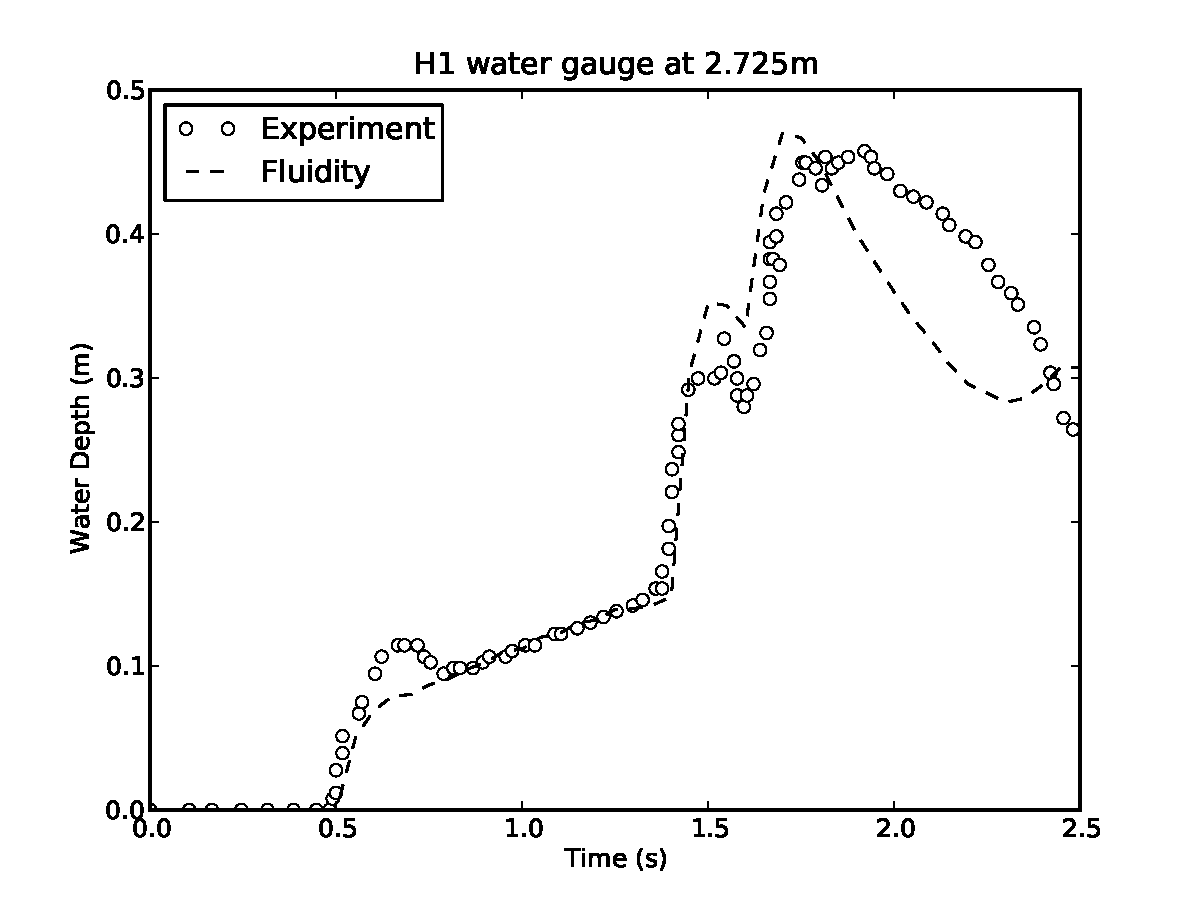
\includegraphics[width=0.75\textwidth]{images/water_gauge_H1.pdf}
\end{frame}


\section{Parallel}
\begin{frame}
    \frametitle{FLML}
No changes required!
\vspace{5mm}

[Optional]
\begin{itemize}
\item Remove fields from stat file
\item Remove some fields from VTU
\end{itemize}
\end{frame}

\begin{frame}
    \frametitle{Decompose mesh}
\vspace{-2mm}
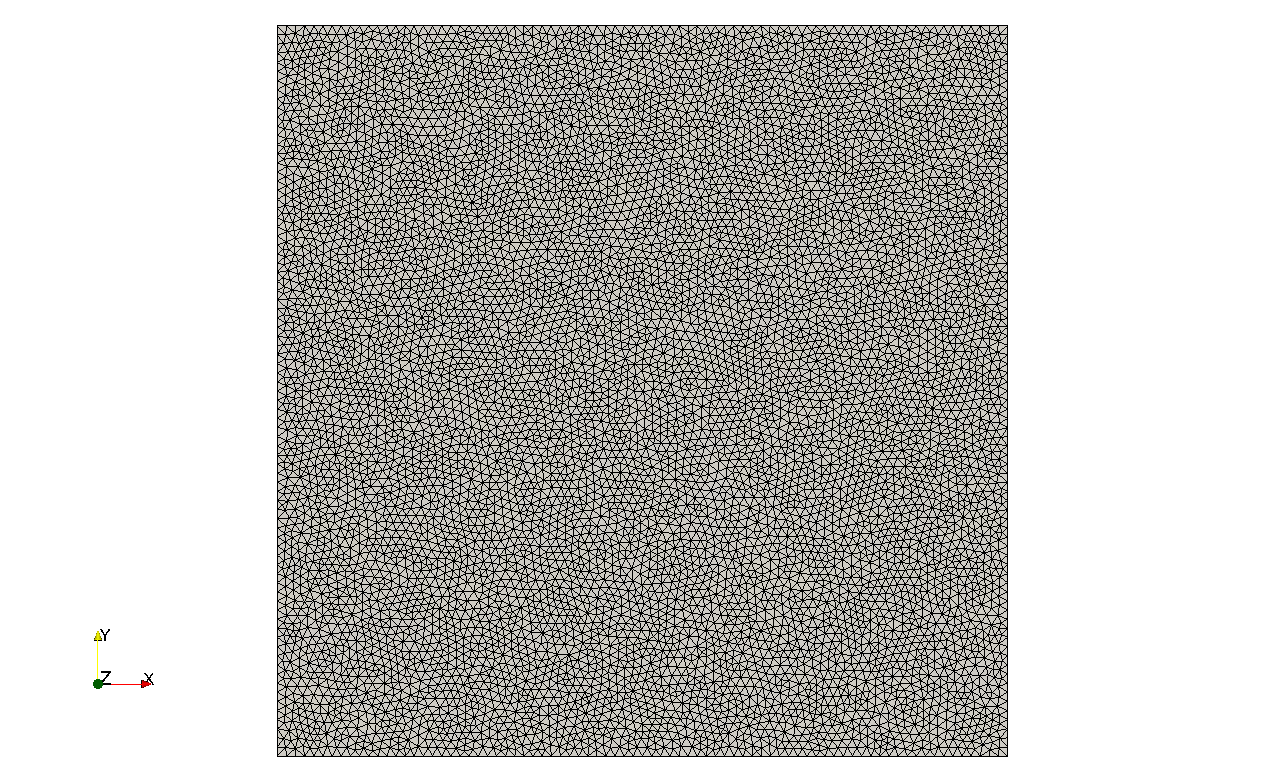
\includegraphics[width=\textwidth]{images/fulldomain.png}
\end{frame}
\begin{frame}
    \frametitle{Decompose mesh}
\vspace{-2mm}
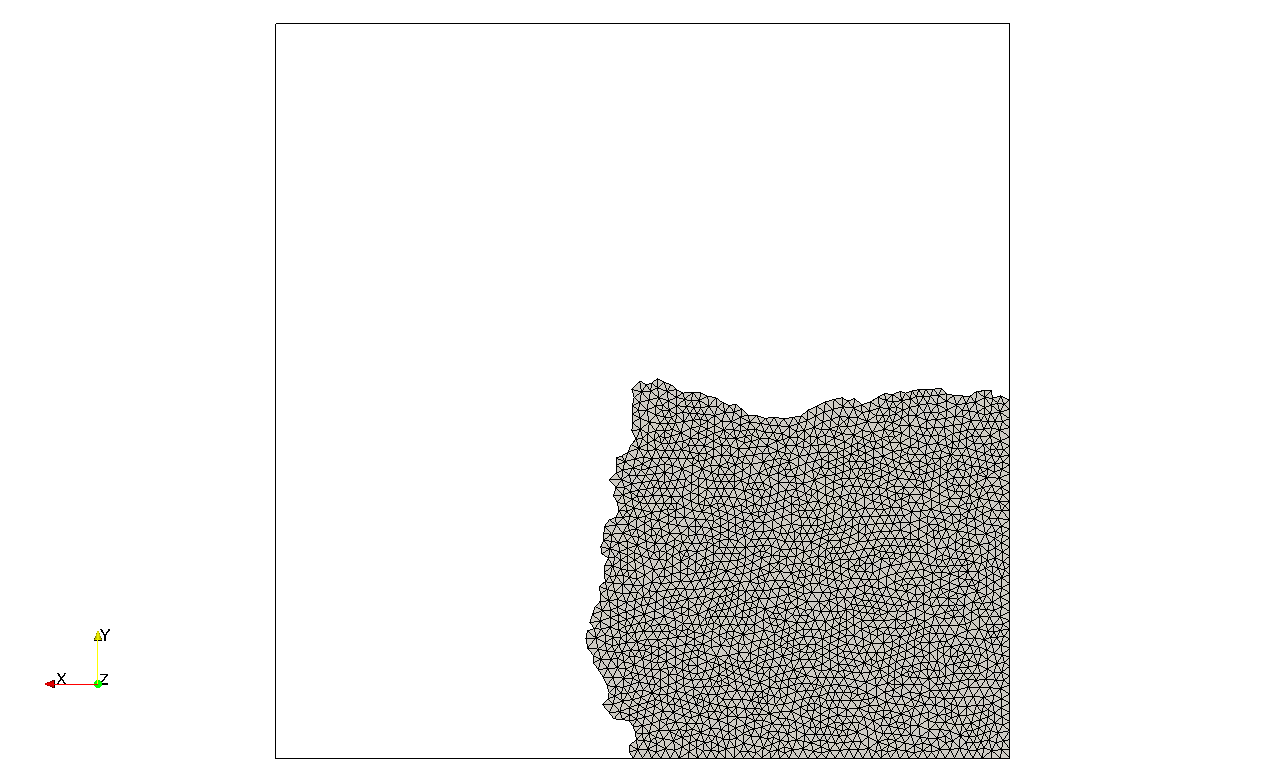
\includegraphics[width=\textwidth]{images/partition1.png}
\end{frame}
\begin{frame}
    \frametitle{Decompose mesh}
\vspace{-2mm}
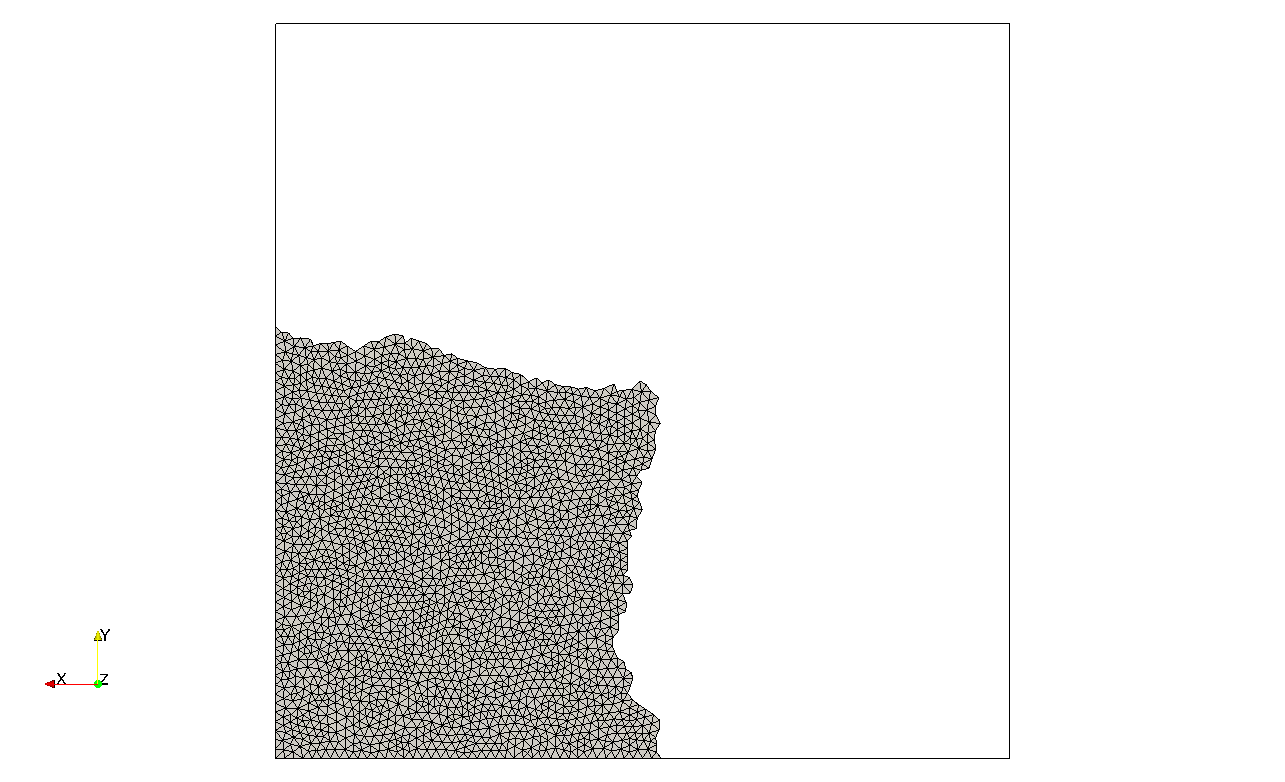
\includegraphics[width=\textwidth]{images/partition2.png}
\end{frame}
\begin{frame}
    \frametitle{Decompose mesh}
\vspace{-2mm}
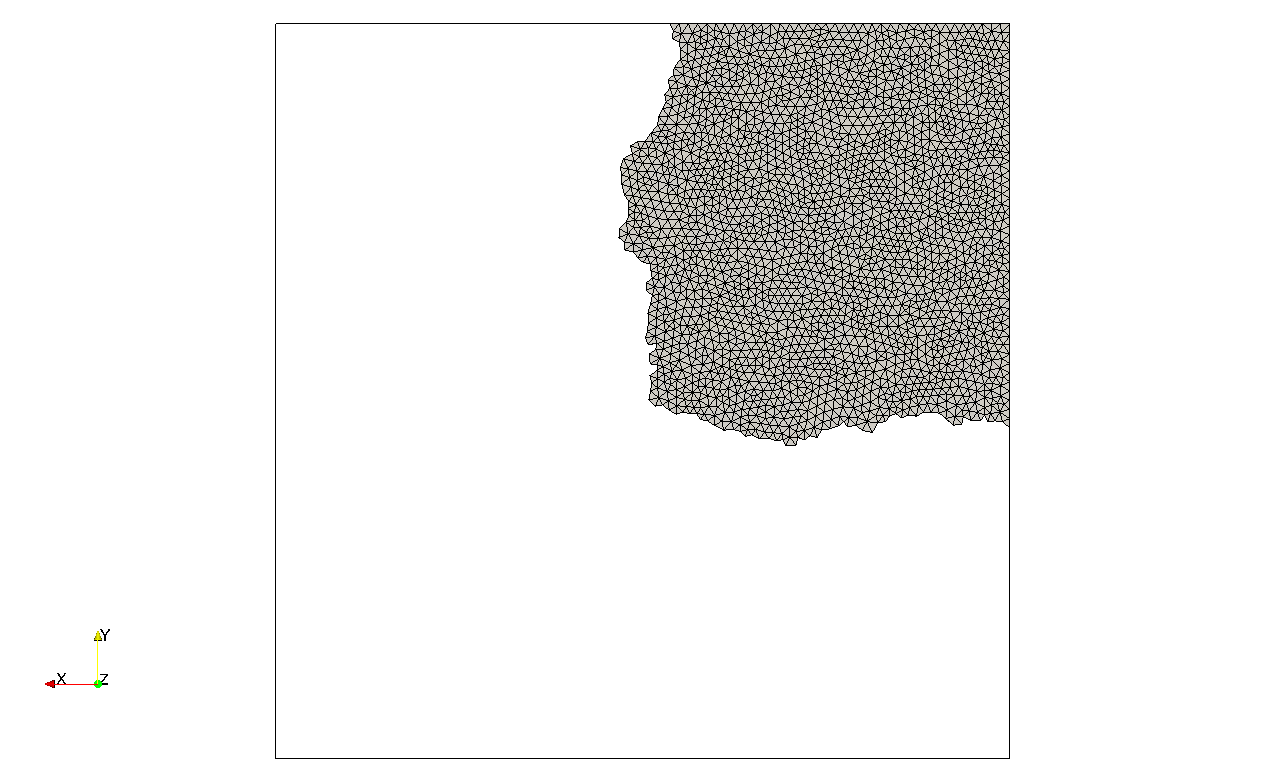
\includegraphics[width=\textwidth]{images/partition3.png}
\end{frame}
\begin{frame}
    \frametitle{Decompose mesh}
\vspace{-2mm}
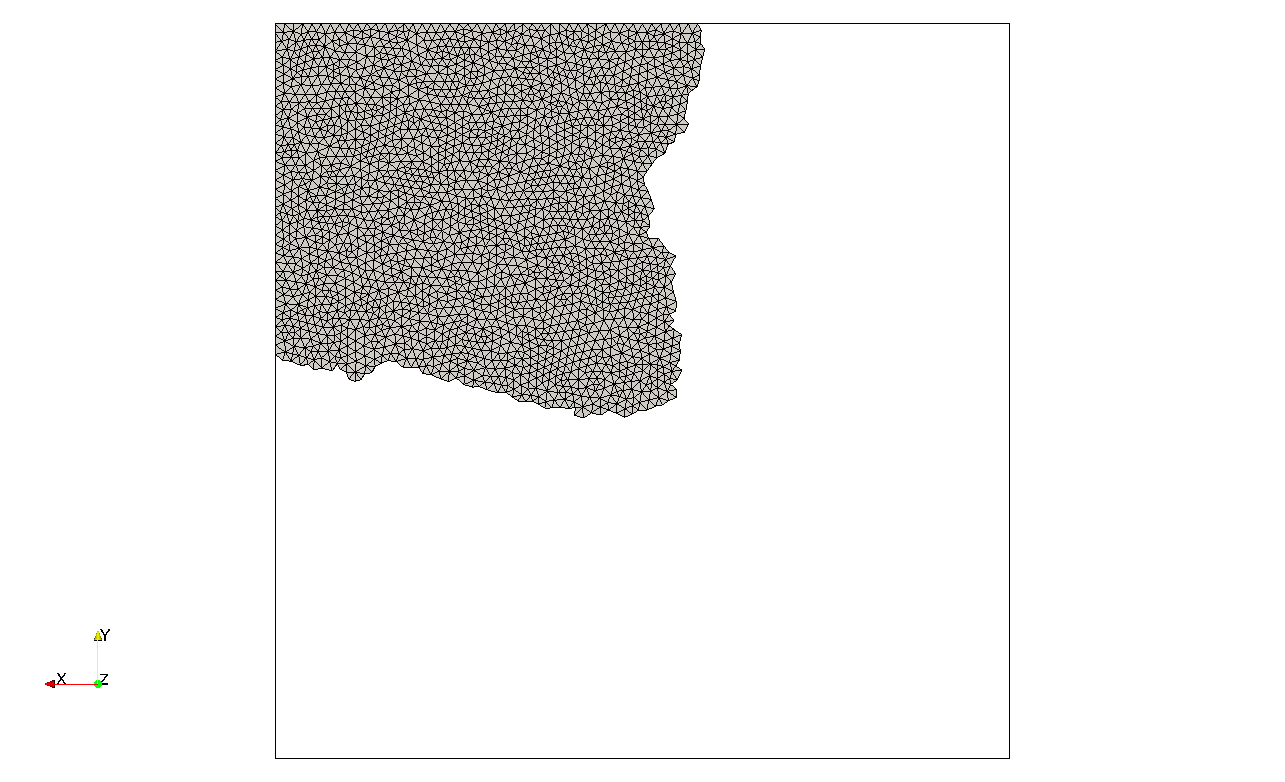
\includegraphics[width=\textwidth]{images/partition4.png}
\end{frame}
\begin{frame}
    \frametitle{Decompose mesh}
\vspace{-2mm}
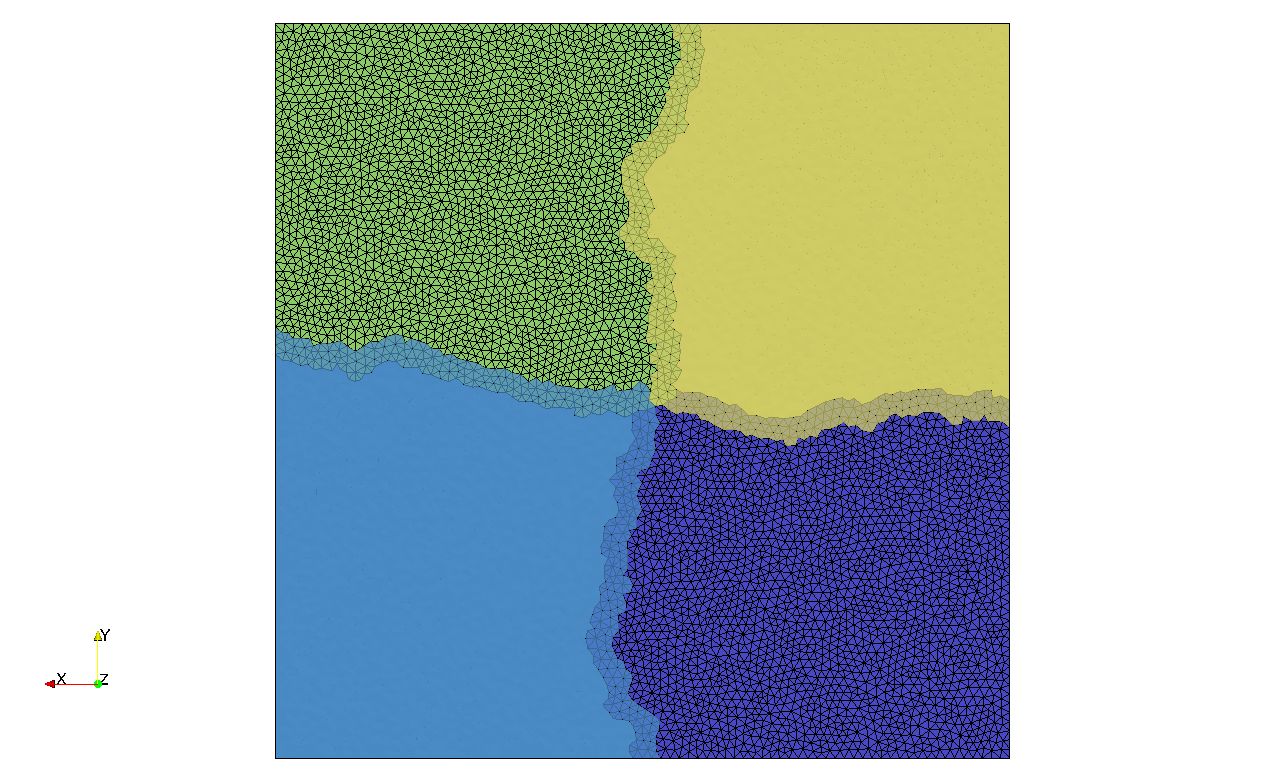
\includegraphics[width=\textwidth]{images/domain_decomp.png}
\end{frame}

\begin{frame}
    \frametitle{\texttt{flredecomp}}
    \scriptsize{\texttt{mpiexec -n 8 flredecomp -i 2 -o 8 InputFLML OutputFLML}}
\vspace{5mm}

Will decompose mesh from 2 to 8.
\vspace{5mm}

\scriptsize{\texttt{mpiexec -n 8 flredecomp -i 8 -o 2 InputFLML OutputFLML}}
\vspace{5mm}

Will decompose mesh from 8 to 2.
\\
Both need running on 8 processors
\\
\textcolor{blue}{\textbf{Note:} Do not add .flml to files, e.g. InputFLML not InputFLML.flml}
\\
\textcolor{blue}{\textbf{Note:} Change of FLML filename to run}
\end{frame}

\subsection{Running}
\begin{frame}
    \frametitle{Local systems}

\texttt{mpiexec -n 8 ../../bin/fluidity my\_flredecomped.flml}
\end{frame}

\subsection{Post-running}
\begin{frame}
    \frametitle{Visualisation}
No different from serial - except .pvtu files, not .vtu
\vspace{5mm}

Log files (if used) will be one per processor.
\end{frame}


\end{document}

